\chapter{Use Cases}

\section{Use Case: Real-Time Moderation}
\label{chap:moderation}
Moderation combines representation, imbalanced classification, thresholds, cascades and human escalation.
The model is therefore one component inside a risk-routing policy.

\subsection{The moderation system is a cascade}
\label{sec:moderation-cascade}
A useful production architecture routes obvious cases cheaply and reserves expensive reasoning for ambiguous or high-impact cases.

\begin{figure}[htbp]
\centering
\resizebox{\linewidth}{!}{%
\begin{tikzpicture}[node distance=7mm and 10mm]
\node[flow] (content) {Text / image\\content};
\node[flow,right=of content] (cheap) {Cheap first-pass\\moderator};
\node[decisionnode,right=of cheap] (risk) {risk /\\uncertainty};
\node[yesbox,above right=6mm and 12mm of risk] (allow) {Clearly safe\\allow};
\node[yesbox,right=18mm of risk] (action) {Clearly severe\\policy action};
\node[flow,below right=6mm and 12mm of risk] (strong) {Stronger\\model};
\node[decisionnode,right=of strong] (amb) {still\\uncertain?};
\node[yesbox,right=of amb] (human) {Human\\review};
\draw[arr] (content)--(cheap);\draw[arr] (cheap)--(risk);
\draw[arr] (risk)--(allow);\draw[arr] (risk)--(action);\draw[arr] (risk)--(strong);
\draw[arr] (strong)--(amb);\draw[arr] (amb)--(human);
\end{tikzpicture}}
\caption{Moderation is a routing system: thresholding and escalation policy determine which model or human sees each case.}
\end{figure}

The cascade idea is the same one developed in \cref{sec:inference-cascades}.
The difference is the cost function: moderation can make false negatives and false positives operationally asymmetric.

\subsection{Text and image representations}
\label{sec:moderation-representations}
Text moderation can use a pretrained Transformer encoder followed by a sequence-level classification head.
Image moderation can use a language-aligned visual representation such as a CLIP-like encoder or a self-supervised visual backbone such as a DINO-like encoder (\cref{sec:cnn-pretrained-visual-representations}).
The practical question is not which name is newer, but whether the pretraining signal makes the harmful/benign distinction easy to express with limited target labels.

For multimodal systems, keep the representation question separate from the final decision policy:
\[
\text{text evidence}
+
\text{image evidence}
+
\text{context}
\rightarrow
\text{risk score}
\rightarrow
\text{threshold/escalation}.
\]

\subsection{Class imbalance: accuracy can be meaningless}
\label{sec:moderation-imbalance}
If $99\%$ of examples are negative, an always-negative classifier obtains $99\%$ accuracy while detecting nothing.
This is why the rare-event metric discussion in \cref{sec:evaluation-precision-recall-and-f1,sec:evaluation-roc-curves-auc-roc-and-precision-recall} matters directly.

\subsubsection{Class weighting versus focal loss}
\label{subsec:moderation-focal}
Weighted cross-entropy changes the cost by class:
\[
\underbrace{\mathcal L_{\text{weighted}}}_{\text{asymmetric class cost}}
=
-\underbrace{w_+y\log p}_{\text{positive errors}}
-\underbrace{w_-(1-y)\log(1-p)}_{\text{negative errors}}.
\]
Focal loss instead downweights examples that are already easy:
\[
\boxed{
\underbrace{\mathcal L_{\text{focal}}}_{\text{focus on hard examples}}
=
-\underbrace{(1-p_{\text{correct}})^\gamma}_{\text{near zero when already easy}}
\log p_{\text{correct}}.
}
\]
The mechanisms are different:
\[
\boxed{
\text{class weighting: some classes matter more}
\qquad
\text{focal loss: easy examples matter less}.
}
\]
Synthetic oversampling such as SMOTE can be useful in some low-dimensional tabular settings but does not automatically create realistic rare examples in complex text/image representation spaces.

\begin{calloutmemoryhook}
Class weighting changes class cost; focal loss reduces the influence of easy examples.
\end{calloutmemoryhook}

\subsection{Thresholds encode the product cost}
\label{sec:moderation-thresholds}
A score becomes an action only after a threshold or routing rule.
Lower thresholds flag more content and typically increase recall while creating more false alarms.
Higher thresholds reduce interventions but miss more positives.
The correct operating point therefore depends on
\[
\boxed{
C_{\text{miss}}
,\quad
C_{\text{false alarm}}
,\quad
C_{\text{human review}}
}.
\]
This is exactly the deployment-threshold separation from \cref{sec:evaluation-decision-thresholds}.

\begin{calloutpractical}
Report the precision--recall operating curve and choose thresholds from the real consequences of misses, interventions and review capacity rather than from accuracy.
\end{calloutpractical}

\subsection{Human review is an expensive model tier}
\label{sec:moderation-human}
Human reviewers are flexible but slow and costly.
A good routing policy therefore concentrates them on cases with high uncertainty, disagreement or impact rather than sampling only the easiest high-confidence examples.
Reviewer decisions can also become future labels, creating the same closed-loop data concerns developed for personalisation in \cref{sec:personalisation-feedback-loop}.

\subsection{Degrees of experiment}
\label{sec:moderation-optionality}
\begin{calloutdegreeofexperiment}
Vary text/image/multimodal representation, loss weighting, focal parameter $\gamma$, sampling policy, thresholds, cascade gate, temporal/context history, human-routing policy and which uncertain cases are labelled for retraining.
\end{calloutdegreeofexperiment}

\begin{calloutmemoryhook}
Moderation quality is the model + threshold + escalation policy.
\end{calloutmemoryhook}

\section{Use Case: Ranking Systems}
\label{chap:ranking}
Ranking at scale is a computational funnel.
Early stages protect recall across huge candidate sets; later stages spend more compute on precise ordering.

\subsection{The ranking funnel}
\label{sec:ranking-funnel}
A representative system shrinks millions of possible items before expensive scoring:
\[
\boxed{
\text{millions}
\rightarrow
\text{retrieval}
\rightarrow
\text{thousands}
\rightarrow
\text{light ranker}
\rightarrow
\text{hundreds}
\rightarrow
\text{heavy reranker}
\rightarrow
\text{final list}
}.
\]

\begin{figure}[htbp]
\centering
\begin{tikzpicture}[node distance=6mm]
\node[flow,minimum width=7.6cm] (all) {Millions of items};
\node[flow,below=of all,minimum width=6.4cm] (retr) {Embedding / ANN retrieval};
\node[flow,below=of retr,minimum width=5.2cm] (light) {Light ranker};
\node[flow,below=of light,minimum width=4.0cm] (heavy) {Heavy reranker};
\node[yesbox,below=of heavy,minimum width=2.8cm] (final) {Displayed list};
\draw[arr] (all)--(retr);\draw[arr] (retr)--(light);\draw[arr] (light)--(heavy);\draw[arr] (heavy)--(final);
\end{tikzpicture}
\caption{Ranking systems spend progressively more modelling capacity on progressively fewer candidates.}
\end{figure}

The same broad design appears in RAG (\cref{sec:llms-rag}): cheap high-recall retrieval first, expensive precision later.

\subsection{Retrieval with two towers}
\label{sec:ranking-retrieval}
A two-tower model computes user/query and item representations independently:
\[
\underbrace{z_{\text{user}}}_{\text{online}}
=f_{\theta}(\text{user, context}),
\qquad
\underbrace{z_{\text{item}}}_{\text{precomputable}}
=g_{\phi}(\text{item}),
\]
then scores compatibility through
\[
\underbrace{s_{\text{retrieve}}}_{\text{ANN-compatible score}}
=
z_{\text{user}}^\top z_{\text{item}}.
\]
Because item vectors can be precomputed, nearest-neighbour search can reduce millions of items to a candidate set.
The embedding/search geometry is developed in \cref{sec:representation-embeddings-as-operational-geometry,subsec:llms-ann}.

\begin{figure}[htbp]
\centering
\begin{tikzpicture}[node distance=8mm and 13mm]
\node[flow] (u) {User +\\context};
\node[flow,below=13mm of u] (i) {Item\\features};
\node[flow,right=of u] (ue) {User\\encoder};
\node[flow,right=of i] (ie) {Item\\encoder};
\node[yesbox,right=of ue] (uv) {User vector};
\node[yesbox,right=of ie] (iv) {Item vector};
\node[flow,right=18mm of uv] (dot) {Dot-product\\compatibility};
\node[yesbox,right=of dot] (cand) {Candidate\\items};
\draw[arr] (u)--(ue);\draw[arr] (i)--(ie);
\draw[arr] (ue)--(uv);\draw[arr] (ie)--(iv);
\draw[arr] (uv)--(dot);\draw[arr] (iv)--(dot);
\draw[arr] (dot)--(cand);
\end{tikzpicture}
\caption{Two-tower retrieval buys scalability by forcing each side to be compressed before user--item interaction.}
\end{figure}

\begin{calloutbias}
If user--item compatibility can be usefully compressed into separate embeddings, two-tower retrieval scales to large catalogues; interactions that require joint fine-grained features are postponed to later rankers.
\end{calloutbias}

\subsection{Ranking and reranking}
\label{sec:ranking-ranking}
Once the candidate set is small enough, a ranker can use richer cross-features:
\[
\underbrace{s_i}_{\text{ranking score}}
=
f(
\text{user},
\text{item}_i,
\text{context},
\text{cross-features}
).
\]
Pointwise, pairwise and listwise objectives were introduced in \cref{sec:objectives-ranking-and-preference-objectives}.
A heavy reranker can additionally compare richer text, history or candidate interactions because it now evaluates tens/hundreds rather than millions.

\subsection{Why NDCG is top-heavy}
\label{sec:ranking-ndcg}
NDCG gives each rank a discount approximately proportional to
\[
\frac{1}{\log_2(r+1)}.
\]
\begin{figure}[htbp]
\centering
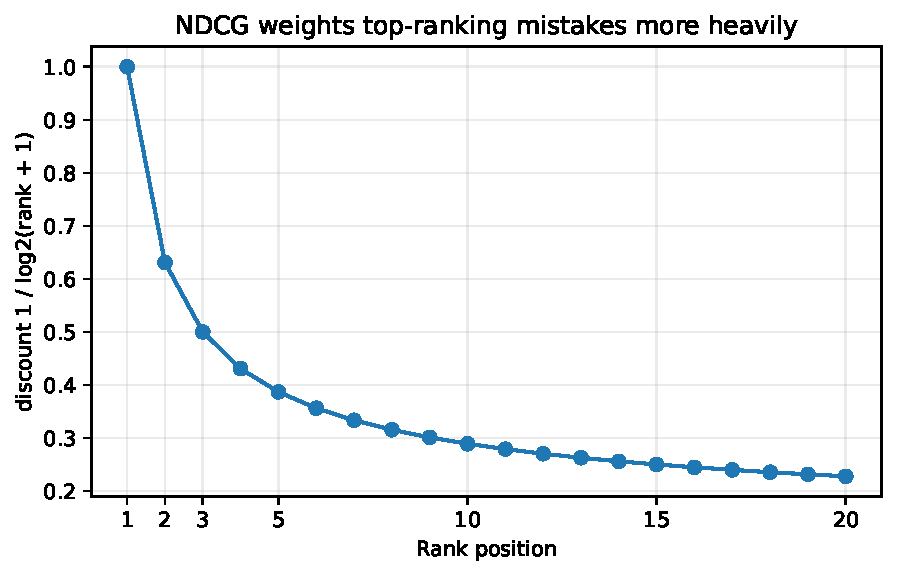
\includegraphics[width=.76\textwidth]{figures/ndcg_discount.pdf}
\caption{The NDCG discount falls fastest at the top, so moving a relevant item between ranks 1 and 2 matters much more than a similar swap deep in the list.}
\label{fig:ranking-ndcg-discount}
\end{figure}
That is why an ordering error near the top can deserve a much stronger training signal than one near rank 100.
LambdaMART uses this idea while retaining boosted-tree stage-wise fitting; see \cref{subsec:trees-lambdamart}.

\subsection{Position bias: clicks mix relevance with exposure}
\label{sec:ranking-position-bias}
A top-ranked item gets more opportunity to be examined than a low-ranked item.
Observed clicks therefore combine at least two effects:
\[
\boxed{
P(\text{click})
\approx
\underbrace{P(\text{examined}\mid\text{position})}_{\text{exposure}}
\times
\underbrace{P(\text{click}\mid\text{examined, relevance})}_{\text{preference}}.
}
\]
Training naively on clicks can make ``was shown high'' look like ``was relevant''.

\begin{figure}[htbp]
\centering
\begin{tikzpicture}[node distance=7mm and 10mm]
\node[flow] (rel) {True relevance};
\node[flow,below=12mm of rel] (pos) {Display position};
\node[yesbox,right=18mm of rel] (click) {Observed click};
\draw[arr] (rel)--(click);
\draw[arr] (pos)--(click);
\end{tikzpicture}
\caption{Click labels are confounded by both user preference and the system's exposure policy.}
\end{figure}

\subsection{Inverse propensity scoring}
\label{sec:ranking-ips}
If the logging policy exposes an item with probability $p_i$, inverse propensity scoring (IPS) weights its observed contribution by roughly
\[
\boxed{
w_i
=
\frac{1}{p_i}.
}
\]
Rarely exposed observations count more because they represent a larger set of opportunities that were usually not shown.
The correction can have high variance:
\[
p_i\rightarrow0
\quad\Rightarrow\quad
w_i\rightarrow\infty.
\]
Practical systems therefore need credible propensity estimates plus clipping/regularisation or explicit exploration where appropriate.

\begin{calloutmemoryhook}
IPS makes rare exposures count more; tiny propensities can make variance explode.
\end{calloutmemoryhook}

\subsection{Evaluation: diagnose the funnel stage}
\label{sec:ranking-evaluation}
Use Recall@K for candidate generation, NDCG/MRR for ordering, and online experiments for product outcomes.
These metrics are defined in \cref{sec:evaluation-retrieval-and-ranking-metrics,sec:evaluation-online-experiments-and-ab-testing}.
Offline ranking gains do not guarantee online user-value gains because historical labels were generated under an earlier exposure policy.

Interleaving can combine results from two rankers into one list for a sensitive direct comparison under the same user/context.
A/B tests remain necessary when the question is broader product impact rather than relative list preference.

\subsection{Degrees of experiment}
\label{sec:ranking-optionality}
\begin{calloutdegreeofexperiment}
Vary candidate sources, user/item representation, embedding dimension, ANN index, candidate count, ranker family, pointwise/pairwise/listwise objective, bias correction, reranker capacity, exploration policy and stage-specific metrics.
\end{calloutdegreeofexperiment}

\begin{calloutmemoryhook}
Retrieve for recall; rank for order; rerank for precision.
\end{calloutmemoryhook}

\section{Use Case: Personalisation}
\label{chap:personalisation}
Ranking asks which item should come first.
Personalisation makes the score depend on who the user is, what the item is, the current context and recent/long-term history:
\[
\boxed{
s
=
f(
\text{user},
\text{item},
\text{context},
\text{history}
).
}
\]

\subsection{From interaction matrix to latent preference space}
\label{sec:personalisation-matrix-factorisation}
Collaborative filtering begins from a sparse user--item interaction matrix.
Matrix factorisation approximates it with low-dimensional user and item vectors:
\[
\underbrace{R}_{N_{\text{users}}\times N_{\text{items}}}
\approx
\underbrace{U}_{N_{\text{users}}\times N_{\text{latent dims}}}
\underbrace{V^\top}_{N_{\text{latent dims}}\times N_{\text{items}}},
\qquad
\underbrace{\hat r_{u,i}}_{\text{predicted preference}}
=
z_u^\top z_i.
\]
The low-rank prerequisite is in \cref{sec:foundations-eigenstructure-and-low-rank-structure}.

\begin{figure}[htbp]
\centering
\begin{tikzpicture}[node distance=8mm and 13mm]
\node[flow] (user) {User ID};
\node[yesbox,right=of user] (uv) {Latent user\\vector};
\node[flow,below=14mm of user] (item) {Item ID};
\node[yesbox,right=of item] (iv) {Latent item\\vector};
\node[flow,right=18mm of uv] (dot) {Dot product};
\node[yesbox,right=of dot] (score) {Preference\\score};
\draw[arr] (user)--(uv);\draw[arr] (item)--(iv);
\draw[arr] (uv)--(dot);\draw[arr] (iv)--(dot);\draw[arr] (dot)--(score);
\end{tikzpicture}
\caption{Matrix factorisation compresses sparse user--item behaviour into a shared latent geometry.}
\end{figure}

\begin{calloutbias}
If user--item preferences have low-dimensional latent structure, matrix factorisation shares statistical strength across sparse interactions; idiosyncratic preferences outside that structure are harder to represent.
\end{calloutbias}

\subsection{Two towers generalise stored latent vectors}
\label{sec:personalisation-two-tower}
A stored user/item vector cannot naturally explain a new identity with no interaction history.
Two-tower models replace lookup-only representations with learned functions:
\[
z_{\text{user}}
=
f_\theta(\text{history, session, context}),
\qquad
z_{\text{item}}
=
g_\phi(\text{text, image, metadata}).
\]
This connects personalisation directly to the retrieval mechanism in \cref{sec:ranking-retrieval}.
Content features let new items acquire a useful representation before many collaborative interactions exist.

\subsection{Cold start: combine collaborative and content evidence}
\label{sec:personalisation-cold-start}
New users/items have little collaborative signal.
Useful fallbacks include content encoders, popularity priors, onboarding choices and rapidly updated session features.
The system therefore often moves from
\[
\text{collaborative only}
\quad\rightarrow\quad
\boxed{\text{collaborative + content + context}}.
\]
The exact mixture can change as interaction history accumulates.

\subsection{Long-term preference versus session intent}
\label{sec:personalisation-timescales}
A user can have stable months-long interests while exhibiting a very different current-session goal.
One representation can therefore combine multiple timescales:
\[
\underbrace{z_{\text{user now}}}_{\text{current preference state}}
=
f(
\underbrace{z_{\text{long-term}}}_{\text{persistent preference}},
\underbrace{z_{\text{session}}}_{\text{current intent}},
\underbrace{\text{context}}_{\text{time/device/location-like context}}
).
\]
Streaming is valuable when the session state changes faster than the model parameters need to be retrained.

\subsection{Temporal decay: encode how quickly preference becomes stale}
\label{sec:personalisation-temporal-decay}
A simple recency rule weights old interactions less:
\[
\boxed{
\underbrace{w(\Delta t)}_{\text{interaction weight}}
=
2^{-\Delta t/\underbrace{T_{1/2}}_{\text{behaviour half-life}}}.
}
\]
\figpdf[.76\textwidth]{temporal_decay}{Different half-lives encode different assumptions about how quickly past behaviour stops predicting current intent.}
A small $T_{1/2}$ forgets quickly; a large one gives long-term history more influence.
The correct decay rate is domain-dependent rather than a universal recommendation.

\begin{calloutbias}
If recent behaviour predicts current intent better than old behaviour, temporal decay is useful; stable long-term preferences can make aggressive decay throw away signal.
\end{calloutbias}

\subsection{The recommendation feedback loop}
\label{sec:personalisation-feedback-loop}
A recommender changes what the user sees, and those exposures create the interaction data used to train its successor.
The data distribution is therefore partly policy-generated:
\[
\boxed{
P(\text{future training data})
=
P(
\text{observations}
\mid
\text{deployed recommender}
).
}
\]

\begin{figure}[htbp]
\centering
\begin{tikzpicture}[node distance=7mm and 9mm]
\node[flow] (rec) {Recommender};
\node[flow,right=of rec] (show) {Chooses\\exposure};
\node[flow,right=of show] (user) {User\\interaction};
\node[flow,right=of user] (logs) {Logged\\data};
\node[flow,right=of logs] (train) {Next training\\dataset};
\draw[arr] (rec)--(show);\draw[arr] (show)--(user);\draw[arr] (user)--(logs);\draw[arr] (logs)--(train);
\draw[arr,rounded corners] (train.south)--++(0,-.75)--([yshift=-.75cm]rec.south)--(rec.south);
\end{tikzpicture}
\caption{Personalisation is a closed-loop system: current recommendations help generate future labels.}
\end{figure}

\subsection{Popularity bias and self-reinforcement}
\label{sec:personalisation-popularity}
Popular items are exposed more, receive more interactions, become easier to estimate, and can then be scored even higher:
\[
\text{popularity}
\rightarrow
\text{exposure}
\rightarrow
\text{interactions}
\rightarrow
\text{training signal}
\rightarrow
\text{future exposure}.
\]
This does not prove popularity is undesirable; it means observed popularity partly reflects the system that generated exposure.
Position-bias correction in \cref{sec:ranking-position-bias,sec:ranking-ips} addresses one part of this general feedback problem.

\subsection{Exploration versus exploitation}
\label{sec:personalisation-exploration}
Always selecting the current highest score exploits existing knowledge but can prevent the system from learning about underexposed alternatives.
Exploration deliberately spends some immediate reward to gain information:
\[
\underbrace{\text{exploit}}_{\text{best current estimate}}
\quad\longleftrightarrow\quad
\underbrace{\text{explore}}_{\text{learn uncertain alternatives}}.
\]
Without exploration, ``never shown'' can become ``never observed'' and then ``never learned to be good''.
Bandit methods formalise this trade-off when actions influence which rewards are observed.

\subsection{Fast state updates versus slow parameter updates}
\label{sec:personalisation-streaming-retraining}
A production recommender often has two update loops:

\begin{figure}[htbp]
\centering
\begin{tikzpicture}[node distance=8mm and 10mm]
\node[flow] (events) {User events};
\node[flow,above right=7mm and 13mm of events] (fast) {Fast stream\\session state};
\node[yesbox,right=of fast] (online) {Online\\ranker};
\node[flow,below right=7mm and 13mm of events] (store) {Historical\\store};
\node[flow,right=of store] (train) {Offline\\retraining};
\node[yesbox,right=of train] (model) {New model\\version};
\draw[arr] (events)--(fast);\draw[arr] (fast)--(online);
\draw[arr] (events)--(store);\draw[arr] (store)--(train);\draw[arr] (train)--(model);
\draw[arr,rounded corners] (model.north)--++(0,.7)--([yshift=.7cm]online.south)--(online.south);
\end{tikzpicture}
\caption{Fast features capture current intent; slower retraining changes the underlying model parameters.}
\end{figure}

A metric drop or drift alert should trigger diagnosis before retraining because data-pipeline failures, inventory changes, delayed labels and real preference shifts need different fixes.
The production-system monitoring stack in \cref{sec:systems-monitoring,sec:systems-drift-retraining} provides the broader framework.

\subsection{Degrees of experiment}
\label{sec:personalisation-optionality}
\begin{calloutdegreeofexperiment}
Vary user representation, item representation, long-term/session weighting, history window, temporal decay, candidate generation, ranking objective, exploration policy, feature freshness, propensity correction and retraining cadence/trigger.
\end{calloutdegreeofexperiment}

\begin{calloutmemoryhook}
The recommender changes the data that trains the next recommender.
\end{calloutmemoryhook}

\section{Use Case: PDE Solvers}
\label{chap:usecase_pde_solvers}

\section{Use Case: Experimental Sensor Regimes}
\label{sec:sensors}
Suppose we have unlabelled measurements from an experimental apparatus collected across operating conditions, with occasional suspected faults but no trusted regime labels.
The goal could be to describe recurring operating states, identify transitions, or prioritise surprising runs; these are \emph{different output requirements} on the same dataset.

\begin{center}
    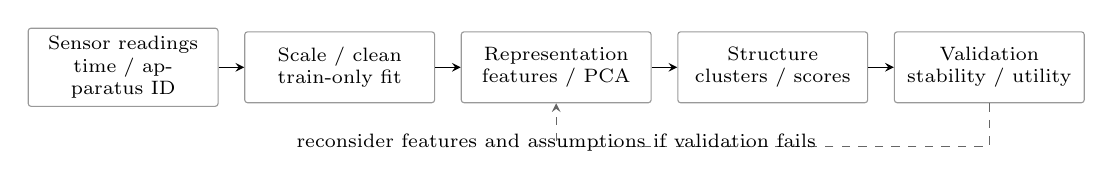
\begin{tikzpicture}[font=\scriptsize,>=stealth]
     \tikzset{ulstage/.style={draw=black!40,rounded corners=1pt,align=center,minimum height=9mm,inner sep=3pt}}
     \node[ulstage,text width=22mm] (raw) at (-5.5,0) {Sensor readings\\time / apparatus ID};
     \node[ulstage,text width=22mm] (prep) at (-2.75,0) {Scale / clean\\train-only fit};
     \node[ulstage,text width=22mm] (rep) at (0,0) {Representation\\features / PCA};
     \node[ulstage,text width=22mm] (model) at (2.75,0) {Structure\\clusters / scores};
     \node[ulstage,text width=22mm] (valid) at (5.5,0) {Validation\\stability / utility};
     \foreach \a/\b in {raw/prep,prep/rep,rep/model,model/valid}{\draw[->] (\a)--(\b);}
     \draw[->,dashed,black!60] (valid.south)--++(0,-.55)-| (rep.south);
     \node[below] at (0,-.72) {reconsider features and assumptions if validation fails};
    \end{tikzpicture}
    \caption{The clustering algorithm is only one stage: feature construction and validation determine whether its structure is meaningful.}
    \label{fig:pipeline}
\end{center}

\textbf{Experimental sequence.}
First, split by time or apparatus where repeated measurements would otherwise leak nearly identical runs across train and validation; fit preprocessing only to the training partition.
Use K-Means as a cheap baseline for compact operating regimes, compare GMM if soft transitions are physically plausible, and test HDBSCAN if groups are curved or rare regimes should remain unassigned.
Compare against hierarchical clustering when understanding sub-regimes at several resolutions matters more than scalability.
If the real requirement is fault triage, compare Isolation Forest and local-density scores against the clustering baselines instead of assuming small clusters are faults.
Inspect whether groups track known nuisance variables (sensor calibration, acquisition batch or ambient temperature) rather than the underlying behaviour of interest.
Finally, freeze the choices and test cluster stability and any downstream fault/retrieval/forecasting gain on unseen data.

\section{Use Case: LLMs}
\label{chap:usecase_LLMs}
\subsection{Training}
\label{sec:modern-llm-training-lifecycle}
Now we have an architecture.
The lifecycle is approximately:

\begin{figure}[htbp]
\centering
\resizebox{.96\linewidth}{!}{%
\begin{tikzpicture}[node distance=7mm and 8mm]
\node[flow] (data) {Internet / books / code / domain data};
\node[flow,right=of data] (clean) {Clean, filter,\\deduplicate};
\node[flow,right=of clean] (tok) {Tokenise};
\node[flow,right=of tok] (pre) {Pretrain};
\node[yesbox,right=of pre] (base) {Base model};
\node[flow,right=of base] (sft) {Supervised\\fine-tuning};
\node[yesbox,right=of sft] (inst) {Instruction\\model};
\node[flow,right=of inst] (pref) {Preference /\\alignment training};
\node[yesbox,right=of pref] (assist) {Assistant};
\draw[arr] (data)--(clean);\draw[arr] (clean)--(tok);\draw[arr] (tok)--(pre);\draw[arr] (pre)--(base);\draw[arr] (base)--(sft);\draw[arr] (sft)--(inst);\draw[arr] (inst)--(pref);\draw[arr] (pref)--(assist);
\end{tikzpicture}}
\caption{The modern LLM training lifecycle: broad predictive pretraining first, then progressively narrower behavioural adaptation.}
\label{fig:modern-llm-training-lifecycle}
\end{figure}

These stages should not be mentally conflated.
The concise versions already appear in \cref{sec:llms-pretraining,sec:llms-sft,sec:llms-preference-optimisation}; here we connect them to the preceding architecture and scaling story.

\subsubsection{Pretraining}
\label{subsec:modern-pretraining}
Consider:
\begin{quote}
The cat sat on the \_\_\_.
\end{quote}

The model predicts a probability distribution, for example:
\begin{center}
\small
\begin{tabular}{lr}
\toprule
Token & Probability \\
\midrule
mat & $0.42$ \\
floor & $0.18$ \\
chair & $0.10$ \\
moon & $0.0001$ \\
\bottomrule
\end{tabular}
\end{center}

During causal-language-model pretraining, we minimise
\[
\mathcal L
=
-\sum_t
\log p_{\theta_{\text{weights}}}(x_t\mid x_{<t}).
\]

Meaning:

\begin{quote}
Assign high probability to the actual next token.
\end{quote}

The data flow is:
\[
[x_1,x_2,x_3,x_4,x_5]
\rightarrow
\underbrace{[x_1,x_2,x_3,x_4]}_{\text{model inputs}}
\rightarrow
\underbrace{[x_2,x_3,x_4,x_5]}_{\text{targets}}.
\]

One sequence gives many predictions simultaneously during training, while causal masking ensures each position sees only valid history.

\textbf{Why next-token prediction learns so much.}
To predict ``The capital of France is \_\_\_'' you need geographical associations.
To predict \code{for i in range(} you benefit from programming syntax.
To predict a detective novel, you benefit from discourse structure and character relationships.

So a very simple objective forces the network to learn whatever statistical structure helps reduce prediction error.
That is one reason language modelling scales surprisingly far.

\paragraph*{Pretraining is not instruction following}
Imagine the input:
\begin{quote}
What is photosynthesis?
\end{quote}

A pure pretrained model has learned:

\begin{quote}
What text probably follows this string?
\end{quote}

It has not necessarily learned the social convention:

\begin{quote}
Produce a concise, useful answer to the user's question.
\end{quote}

That is a different behavioural objective.
Hence post-training.

\subsubsection{Fine-tuning}
\label{subsec:modern-finetuning}
Fine-tuning begins with pretrained parameters
\[
\theta_{\text{pretrained weights}}
\]
and continues training on a narrower dataset.

For instruction tuning:
\[
\underbrace{\text{``Explain gradient descent simply.''}}_{\text{input}}
\longrightarrow
\underbrace{\text{``Gradient descent is...''}}_{\text{target}}.
\]

The resulting gradient updates the pretrained model toward this desired interaction pattern.

\begin{center}
\small
\begin{tabularx}{.91\linewidth}{@{}L{.22\linewidth}YY@{}}
\toprule
 & \textbf{Pretraining} & \textbf{Fine-tuning} \\
\midrule
Data & huge / general & smaller / specialised \\
Goal & learn broad distribution & adapt behaviour/domain/task \\
Cost & enormous & much smaller \\
Starting point & random-ish parameters & pretrained model \\
Output & base model & adapted model \\
\bottomrule
\end{tabularx}
\end{center}

Fine-tuning works because the expensive representational learning already occurred.

\begin{calloutintuition}
Pretraining is the broad education; fine-tuning is learning the specific behaviour and methods needed in one lab or role.
\end{calloutintuition}

\subsubsection{The problem with full fine-tuning}
\label{subsec:modern-full-ft-cost}
Suppose your base model has 70 billion parameters.
Full fine-tuning potentially updates all 70B.
During Adam-like optimisation you may need storage associated with weights, gradients, first moments and second moments.
This becomes very expensive.

And if you want 100 specialised versions, storing 100 complete parameter copies is cumbersome.
That motivates parameter-efficient fine-tuning.
\paragraph{Fine Tuning}LoRA begins with a pretrained weight matrix $\theta_{\text{weights}}$.
Ordinary fine-tuning learns a full update:
\[
\theta'_{\text{weights}}
=
\theta_{\text{weights}}+\Delta\theta.
\]

If
\[
\theta_{\text{weights}}
\in
\mathbb{R}^{N_{\text{output features}}\times N_{\text{input features}}},
\]
then a full $\Delta\theta$ potentially contains
\[
N_{\text{output features}}N_{\text{input features}}
\]
learnable numbers.

LoRA says:

\begin{quote}
Perhaps the useful adaptation lives in a much lower-dimensional subspace.
\end{quote}

Represent the update as
\[
\boxed{
\Delta\theta
=
\theta_{\text{up}}\theta_{\text{down}}
}
\]
where
\[
\theta_{\text{down}}
\in
\mathbb{R}^{N_{\text{adaptation directions}}\times N_{\text{input features}}},
\]
\[
\theta_{\text{up}}
\in
\mathbb{R}^{N_{\text{output features}}\times N_{\text{adaptation directions}}},
\]
and
\[
N_{\text{adaptation directions}}
\ll
N_{\text{input/output features}}.
\]

The base matrix is frozen.
Only the low-rank factors are trained.
This same mechanism is developed in \cref{sec:adaptation-lora-a-parameter-efficient-adaptation-mechanism}; the linear-algebra prerequisite is \cref{subsec:la-span-and-rank}.

\textbf{Why this saves parameters.}
Suppose
\[
\theta_{\text{weights}}
\in
\mathbb{R}^{4096\times4096}.
\]

A full update contains
\[
4096^2=16.8\text{ million parameters}.
\]

LoRA with
\[
N_{\text{adaptation directions}}=8
\]
needs
\[
4096\times8+8\times4096=65{,}536
\]
trainable numbers for that matrix: roughly $256\times$ fewer.

\textbf{LoRA intuition.}
Imagine a full matrix update can change a representation in every conceivable direction.
LoRA says that adapting from ``general language model'' to a particular downstream behaviour may require only a small number of important directions in parameter space.

\begin{calloutbias}
If useful downstream adaptation is approximately low-rank, freezing the base and learning a small low-rank update captures much of the required change; if the task requires many independent adaptation directions, too small a rank becomes restrictive.
\end{calloutbias}

\begin{calloutdegreeofexperiment}
For LoRA, vary rank, update scaling, target modules, dropout, which layers receive adapters and the adaptation dataset.
\end{calloutdegreeofexperiment}

\begin{calloutpractical}
LoRA is a fine-tuning method, not a new Transformer architecture.
At inference, compatible LoRA updates can often be merged into the base matrix as $\theta'_{\text{weights}}=\theta_{\text{weights}}+\theta_{\text{up}}\theta_{\text{down}}$.
\end{calloutpractical}

\subsubsection{RLHF}
\label{subsec:modern-rlhf}
Now suppose supervised fine-tuning gives two answers: one technically correct but unhelpful, and one correct, concise, clear and instruction-following.
Maximum-likelihood SFT only directly trains on provided target responses.
But humans can often more easily say:

\begin{quote}
B is better than A.
\end{quote}

RLHF uses preference information.
The classic pipeline is:

\begin{figure}[htbp]
\centering
\resizebox{.94\linewidth}{!}{%
\begin{tikzpicture}[node distance=7mm and 8mm]
\node[flow] (sft) {1. Supervised\\fine-tuning};
\node[flow,right=of sft] (gen) {Generate several\\candidate answers};
\node[flow,right=of gen] (rank) {Humans rank\\candidates};
\node[flow,right=of rank] (reward) {2. Train reward /\\preference model};
\node[flow,right=of reward] (rl) {3. Optimise\\language-model policy};
\draw[arr] (sft)--(gen);\draw[arr] (gen)--(rank);\draw[arr] (rank)--(reward);\draw[arr] (reward)--(rl);
\end{tikzpicture}}
\caption{Classical RLHF: demonstrations first, then human rankings, then policy optimisation against the learned preference signal.}
\label{fig:modern-rlhf-pipeline}
\end{figure}

The existing broader preference-optimisation framing is in \cref{sec:llms-preference-optimisation}; the ranking-objective connection is in \cref{sec:objectives-ranking-and-preference-objectives}.

\paragraph*{Reward model intuition}
Suppose humans rank
\[
A>B>C.
\]

Train a model that maps prompt plus response to a scalar preference score:
\[
R_{\theta_{\text{reward}}}(x,y).
\]

For example:
\[
A\rightarrow3.2,
\qquad
B\rightarrow1.1,
\qquad
C\rightarrow-0.7.
\]

These are not objective physical units.
They represent learned human preference.

\paragraph*{Then reinforcement learning}
The language model defines a policy
\[
\pi_{\theta_{\text{weights}}}(y\mid x).
\]

The optimisation pushes it toward outputs with higher learned reward:
\[
\max_{\theta_{\text{weights}}}
\mathbb E[R_{\theta_{\text{reward}}}(x,y)].
\]

But blindly maximising the reward model is dangerous statistically: the policy can exploit imperfections in the learned reward function.
So classical RLHF adds a penalty discouraging the policy from moving too far from a reference model.
Conceptually:
\[
\boxed{
\text{objective}
=
\text{preference reward}
-
\beta\,\text{distance from reference policy}
}.
\]

This gives the optimisation a tether.

\paragraph*{SFT vs RLHF}
SFT says:
\begin{quote}
For this input, imitate this desired answer.
\end{quote}

Preference training says:
\begin{quote}
Between these possible behaviours, humans prefer this one.
\end{quote}

So SFT learns \textbf{demonstrations}.
RLHF learns from \textbf{comparative preferences} and then optimises behaviour against them.
Modern post-training includes additional preference-optimisation approaches, but the classical RLHF pipeline remains the right conceptual foundation.


\subsection{Reasoning}
\subsubsection{Reasoning in Latent Space}


\subsection{Prompting, RAG and fine-tuning solve different missing pieces}
\label{sec:llms-prompt-rag-ft}
Choose the intervention according to what must change.

\begin{figure}[htbp]
\centering
\begin{tikzpicture}[node distance=7mm and 10mm]
\node[decisionnode] (q) {What is\\missing?};
\node[yesbox,above right=9mm and 18mm of q] (prompt) {Temporary instruction\\or small context\\$\rightarrow$ prompt};
\node[yesbox,right=25mm of q] (rag) {Changing/private facts\\$\rightarrow$ RAG};
\node[yesbox,below right=9mm and 18mm of q] (ft) {Persistent behaviour\\$\rightarrow$ SFT / LoRA};
\draw[arr] (q)--(prompt);
\draw[arr] (q)--(rag);
\draw[arr] (q)--(ft);
\end{tikzpicture}
\caption{Prompting changes the current context, RAG changes accessible evidence, and fine-tuning changes persistent model behaviour.}
\end{figure}

A useful optionality axis is
\[
    \underbrace{\text{prompt}}_{\text{cheap/reversible}}
    \rightarrow
    \text{RAG}
    \rightarrow
    \text{LoRA}
    \rightarrow
    \text{partial fine-tuning}
    \rightarrow
    \underbrace{\text{full fine-tuning}}_{\text{more invasive}}.
\]
The LoRA mechanism is already derived in \cref{sec:adaptation-lora-a-parameter-efficient-adaptation-mechanism}; QLoRA adds a quantised frozen base in \cref{subsec:adaptation-qlora}.

\subsection{RAG: external evidence as an inference-time memory}
\label{sec:llms-rag}
Retrieval-augmented generation (RAG) separates external knowledge from the language-model weights.
Documents are indexed offline; a query retrieves useful chunks online; those chunks become additional context for generation.

\begin{figure}[htbp]
\centering
\resizebox{\linewidth}{!}{%
\begin{tikzpicture}[node distance=7mm and 7mm]
\node[flow] (docs) {Documents};
\node[flow,right=of docs] (chunks) {Chunk};
\node[flow,right=of chunks] (emb) {Embed};
\node[yesbox,right=of emb] (index) {Vector index};
\node[flow,below=13mm of docs] (query) {User query};
\node[flow,right=of query] (rewrite) {Optional\\rewrite};
\node[flow,right=of rewrite] (qemb) {Query\\embedding};
\node[flow,right=of qemb] (retrieve) {Broad ANN\\retrieval};
\node[flow,right=of retrieve] (rerank) {Precise\\reranking};
\node[yesbox,right=of rerank] (context) {Top context\\chunks};
\node[flow,right=of context] (llm) {LLM};
\node[yesbox,right=of llm] (ans) {Answer};
\draw[arr] (docs)--(chunks);\draw[arr] (chunks)--(emb);\draw[arr] (emb)--(index);
\draw[arr] (query)--(rewrite);\draw[arr] (rewrite)--(qemb);\draw[arr] (qemb)--(retrieve);
\draw[arr] (index.south)--(retrieve.north);
\draw[arr] (retrieve)--(rerank);\draw[arr] (rerank)--(context);\draw[arr] (context)--(llm);\draw[arr] (llm)--(ans);
\end{tikzpicture}}
\caption{RAG separates broad cheap retrieval from expensive precise reranking before the language model sees a small evidence set.}
\end{figure}


A conversational query can be rewritten into a search-specific query before embedding, which can improve retrieval when the raw wording depends on chat context.
The rewrite is itself a model choice: an aggressive rewrite can also distort user intent.


\subsubsection{Chunking: choose the unit that retrieval can retrieve}
\label{subsec:llms-chunking}
Very small chunks are specific but can lose surrounding context.
Very large chunks preserve context but dilute the embedding signal and consume more LLM context.
Overlap reduces boundary failures at the cost of index duplication.
Chunking is therefore a modelling choice:
\[
\boxed{
\text{specific retrieval unit}
\longleftrightarrow
\text{complete local context}
}.
\]

\subsubsection{Bi-encoder retrieval versus cross-encoder reranking}
\label{subsec:llms-bi-cross}
A bi-encoder maps query and document separately:
\[
\underbrace{z_{\text{query}}}_{\text{computed online}}
=f_\theta(q),
\qquad
\underbrace{z_{\text{doc}}}_{\text{precomputed}}
=g_\phi(d),
\qquad
\underbrace{s(q,d)}_{\text{cheap compatibility}}
=z_{\text{query}}^\top z_{\text{doc}}.
\]
This supports vector indexing because document vectors can be stored once.
A cross-encoder instead processes query and candidate document together, allowing richer token-level interaction but requiring one expensive pass per candidate.

\begin{center}
\small
\begin{tabularx}{.94\linewidth}{@{}L{.23\linewidth}YY@{}}
\toprule
 & \textbf{Bi-encoder} & \textbf{Cross-encoder} \\
\midrule
Query/document interaction & Compressed into two vectors & Joint token-level interaction \\
Document preprocessing & Precompute vectors & Must score per query--document pair \\
Typical role & High-recall retrieval & Precision reranking \\
Scaling & Millions of candidates & Tens/hundreds of candidates \\
\bottomrule
\end{tabularx}
\end{center}

\begin{calloutmemoryhook}
Retrieve broadly; rerank precisely.
\end{calloutmemoryhook}

\subsubsection{Approximate nearest neighbours: HNSW versus IVF}
\label{subsec:llms-ann}
Exact nearest-neighbour search compares the query with every stored vector.
Approximate nearest-neighbour (ANN) methods trade a small amount of retrieval exactness for much lower search work.

\begin{figure}[htbp]
\centering
\begin{tikzpicture}[node distance=8mm and 18mm]
\node[flow] (h) {HNSW\\navigate a graph\\of nearby vectors};
\node[flow,right=of h] (i) {IVF\\choose coarse regions\\then search inside};
\node[yesbox,below=10mm of h] (ht) {Main knob:\\graph search breadth};
\node[yesbox,below=10mm of i] (it) {Main knob:\\clusters probed};
\draw[arr] (h)--(ht);
\draw[arr] (i)--(it);
\end{tikzpicture}
\caption{HNSW prunes search by graph navigation; IVF prunes search by coarse spatial partitioning.}
\end{figure}

HNSW usually spends extra memory on graph edges and searches by repeatedly moving toward closer neighbours.
IVF first assigns vectors to coarse centroids, then searches only selected cells.
The index choice should be compared on recall, latency, memory and update behaviour rather than by algorithm name alone.

\begin{calloutdegreeofexperiment}
For RAG, vary chunking, embedding model/dimension, similarity, ANN index, number retrieved, reranker, number of chunks placed in context, query rewriting and generation model.
\end{calloutdegreeofexperiment}

\subsection{MultiAgent}

\subsection{Agentic systems: an LLM inside a stateful control loop}
\label{sec:llms-agents}
A tool-using agent is not simply a larger model.
The language model proposes the next step, an orchestrator owns state/branching/stopping, and tools perform external operations.

\begin{figure}[htbp]
\centering
\begin{tikzpicture}[node distance=8mm and 10mm]
\node[flow] (user) {User request};
\node[flow,right=of user] (llm) {LLM\\proposes next step};
\node[decisionnode,right=of llm] (toolq) {need\\tool?};
\node[flow,above right=5mm and 13mm of toolq] (tool) {Tool / API};
\node[yesbox,right=of tool] (obs) {Observation};
\node[yesbox,below right=5mm and 13mm of toolq] (answer) {Final answer};
\draw[arr] (user)--(llm);
\draw[arr] (llm)--(toolq);
\draw[arr] (toolq)--node[above,font=\scriptsize]{yes}(tool);
\draw[arr] (tool)--(obs);
\draw[arr,rounded corners] (obs.north)--++(0,.6)--([yshift=.6cm]llm.north)--(llm.north);
\draw[arr] (toolq)--node[below,font=\scriptsize]{no}(answer);
\end{tikzpicture}
\caption{The orchestrator turns model calls into a loop; tool execution and approval policy remain outside the language model.}
\end{figure}

High-impact actions can include mandatory human approval gates.
That is a stronger systems guarantee than relying on the model to remember a prose instruction.
Tool protocols standardise how external capabilities are exposed; inference engines independently optimise how model calls are served.

\begin{calloutmemoryhook}
An agent is an LLM inside a stateful control loop with tools.
\end{calloutmemoryhook}

\subsection{LLM research optionality}
\label{sec:llms-optionality}
\begin{center}
\small
\begin{tabularx}{.96\linewidth}{@{}L{.22\linewidth}YY@{}}
\toprule
\textbf{Layer} & \textbf{Knobs} & \textbf{What changes} \\
\midrule
Base model & size, context, architecture & raw modelling capacity / cost \\
Adaptation & prompt, SFT, LoRA, full FT & persistent versus temporary behaviour \\
Retrieval & chunking, embedding, ANN, reranking & external evidence quality / latency \\
Context assembly & number/order of chunks & evidence coverage versus context cost \\
Decoding & temperature, top-$p$, stopping & output diversity and latency \\
Tools & available actions / permissions & external capability and risk \\
Orchestration & state, loops, approval gates & control flow and reliability \\
\bottomrule
\end{tabularx}
\end{center}


